\subsection{Implementación con Qiskit}
Para mostrar de forma detallada se trabajara con el problema cuando $a=7$ y $N=15$. Con esto, realizamos el operador U aplicado al estado $\left|y \right\rangle$ de la siguiente manera:
\begin{equation}
    U\left| y \right\rangle = \left|aymod15 \right\rangle 
    \label{eq:ua15}
\end{equation}
Para crear las operaciones acumulativas $U^x$, se creará una repetición del circuito $x$ veces, por lo que la función \textcolor{def}{\textit{c\_amod15}}
 regresará la compuerta U al valor de a y la añadira al circuito cuántico con la función \textcolor{def}{\textit{modular\_exponentiation}}, repetida x veces como lo siguiente:
 \begin{tcolorbox}[breakable, size=fbox, boxrule=1pt, pad at break*=1mm,colback=cellbackground, colframe=cellborder]
    \prompt{In}{incolor}{}{\boxspacing}
    \begin{Verbatim}[commandchars=\\\{\}]
    \PY{k}{def} \PY{n+nf}{c\PYZus{}amod15}\PY{p}{(}\PY{n}{a}\PY{p}{,} \PY{n}{x}\PY{p}{)}\PY{p}{:}
        \PY{k}{if} \PY{n}{a} \PY{o+ow}{not} \PY{o+ow}{in} \PY{p}{[}\PY{l+m+mi}{2}\PY{p}{,}\PY{l+m+mi}{7}\PY{p}{,}\PY{l+m+mi}{8}\PY{p}{,}\PY{l+m+mi}{11}\PY{p}{,}\PY{l+m+mi}{13}\PY{p}{]}\PY{p}{:}
            \PY{k}{raise} \PY{n+ne}{ValueError}\PY{p}{(}\PY{l+s+s2}{\PYZdq{}}\PY{l+s+s2}{\PYZsq{}}\PY{l+s+s2}{a}\PY{l+s+s2}{\PYZsq{}}\PY{l+s+s2}{ debe ser 2,7,8,11 o 13}\PY{l+s+s2}{\PYZdq{}}\PY{p}{)}
        \PY{n}{U} \PY{o}{=} \PY{n}{QuantumCircuit}\PY{p}{(}\PY{l+m+mi}{4}\PY{p}{)}        
        \PY{k}{for} \PY{n}{iteration} \PY{o+ow}{in} \PY{n+nb}{range}\PY{p}{(}\PY{n}{x}\PY{p}{)}\PY{p}{:}
            \PY{k}{if} \PY{n}{a} \PY{o+ow}{in} \PY{p}{[}\PY{l+m+mi}{2}\PY{p}{,}\PY{l+m+mi}{13}\PY{p}{]}\PY{p}{:}
                \PY{n}{U}\PY{o}{.}\PY{n}{swap}\PY{p}{(}\PY{l+m+mi}{0}\PY{p}{,}\PY{l+m+mi}{1}\PY{p}{)}
                \PY{n}{U}\PY{o}{.}\PY{n}{swap}\PY{p}{(}\PY{l+m+mi}{1}\PY{p}{,}\PY{l+m+mi}{2}\PY{p}{)}
                \PY{n}{U}\PY{o}{.}\PY{n}{swap}\PY{p}{(}\PY{l+m+mi}{2}\PY{p}{,}\PY{l+m+mi}{3}\PY{p}{)}
            \PY{k}{if} \PY{n}{a} \PY{o+ow}{in} \PY{p}{[}\PY{l+m+mi}{7}\PY{p}{,}\PY{l+m+mi}{8}\PY{p}{]}\PY{p}{:}
                \PY{n}{U}\PY{o}{.}\PY{n}{swap}\PY{p}{(}\PY{l+m+mi}{2}\PY{p}{,}\PY{l+m+mi}{3}\PY{p}{)}
                \PY{n}{U}\PY{o}{.}\PY{n}{swap}\PY{p}{(}\PY{l+m+mi}{1}\PY{p}{,}\PY{l+m+mi}{2}\PY{p}{)}
                \PY{n}{U}\PY{o}{.}\PY{n}{swap}\PY{p}{(}\PY{l+m+mi}{0}\PY{p}{,}\PY{l+m+mi}{1}\PY{p}{)}
            \PY{k}{if} \PY{n}{a} \PY{o}{==} \PY{l+m+mi}{11}\PY{p}{:}
                \PY{n}{U}\PY{o}{.}\PY{n}{swap}\PY{p}{(}\PY{l+m+mi}{1}\PY{p}{,}\PY{l+m+mi}{3}\PY{p}{)}
                \PY{n}{U}\PY{o}{.}\PY{n}{swap}\PY{p}{(}\PY{l+m+mi}{0}\PY{p}{,}\PY{l+m+mi}{2}\PY{p}{)}
            \PY{k}{if} \PY{n}{a} \PY{o+ow}{in} \PY{p}{[}\PY{l+m+mi}{7}\PY{p}{,}\PY{l+m+mi}{11}\PY{p}{,}\PY{l+m+mi}{13}\PY{p}{]}\PY{p}{:}
                \PY{k}{for} \PY{n}{q} \PY{o+ow}{in} \PY{n+nb}{range}\PY{p}{(}\PY{l+m+mi}{4}\PY{p}{)}\PY{p}{:}
                    \PY{n}{U}\PY{o}{.}\PY{n}{x}\PY{p}{(}\PY{n}{q}\PY{p}{)}
        \PY{n}{U} \PY{o}{=} \PY{n}{U}\PY{o}{.}\PY{n}{to\PYZus{}gate}\PY{p}{(}\PY{p}{)}
        \PY{n}{U}\PY{o}{.}\PY{n}{name} \PY{o}{=} \PY{l+s+s2}{\PYZdq{}}\PY{l+s+si}{\PYZpc{}i}\PY{l+s+s2}{\PYZca{}}\PY{l+s+si}{\PYZpc{}i}\PY{l+s+s2}{ mod 15}\PY{l+s+s2}{\PYZdq{}} \PY{o}{\PYZpc{}} \PY{p}{(}\PY{n}{a}\PY{p}{,} \PY{n}{x}\PY{p}{)}
        \PY{n}{c\PYZus{}U} \PY{o}{=} \PY{n}{U}\PY{o}{.}\PY{n}{control}\PY{p}{(}\PY{p}{)}
        \PY{k}{return} \PY{n}{c\PYZus{}U}
    \PY{k}{def} \PY{n+nf}{modular\PYZus{}exponentiation}\PY{p}{(}\PY{n}{given\PYZus{}circuit}\PY{p}{,} \PY{n}{n}\PY{p}{,} \PY{n}{m}\PY{p}{,} \PY{n}{a}\PY{p}{)}\PY{p}{:}
        \PY{k}{for} \PY{n}{x} \PY{o+ow}{in} \PY{n+nb}{range}\PY{p}{(}\PY{n}{n}\PY{p}{)}\PY{p}{:}
            \PY{n}{exponent} \PY{o}{=} \PY{l+m+mi}{2}\PY{o}{*}\PY{o}{*}\PY{n}{x}
            \PY{n}{given\PYZus{}circuit}\PY{o}{.}\PY{n}{append}\PY{p}{(}\PY{n}{a\PYZus{}x\PYZus{}mod15}\PY{p}{(}\PY{n}{a}\PY{p}{,} \PY{n}{exponent}\PY{p}{)}\PY{p}{,} 
                         \PY{p}{[}\PY{n}{x}\PY{p}{]} \PY{o}{+} \PY{n+nb}{list}\PY{p}{(}\PY{n+nb}{range}\PY{p}{(}\PY{n}{n}\PY{p}{,} \PY{n}{n}\PY{o}{+}\PY{n}{m}\PY{p}{)}\PY{p}{)}\PY{p}{)}
    \end{Verbatim}
    \end{tcolorbox}
Al algortimo también se le implemento la transformación inversa de Fourier cuántica, se le nombre como \textcolor{def}{\textit{qft\_dagger}}, esta función es la siguiente:
\begin{tcolorbox}[breakable, size=fbox, boxrule=1pt, pad at break*=1mm,colback=cellbackground, colframe=cellborder]
    \prompt{In}{incolor}{}{\boxspacing}
    \begin{Verbatim}[commandchars=\\\{\}]
    \PY{k}{def} \PY{n+nf}{qft\PYZus{}dagger}\PY{p}{(}\PY{n}{n}\PY{p}{)}\PY{p}{:}
        \PY{n}{qc} \PY{o}{=} \PY{n}{QuantumCircuit}\PY{p}{(}\PY{n}{n}\PY{p}{)}
        \PY{k}{for} \PY{n}{qubit} \PY{o+ow}{in} \PY{n+nb}{range}\PY{p}{(}\PY{n}{n}\PY{o}{/}\PY{o}{/}\PY{l+m+mi}{2}\PY{p}{)}\PY{p}{:}
            \PY{n}{qc}\PY{o}{.}\PY{n}{swap}\PY{p}{(}\PY{n}{qubit}\PY{p}{,} \PY{n}{n}\PY{o}{\PYZhy{}}\PY{n}{qubit}\PY{o}{\PYZhy{}}\PY{l+m+mi}{1}\PY{p}{)}
        \PY{k}{for} \PY{n}{j} \PY{o+ow}{in} \PY{n+nb}{range}\PY{p}{(}\PY{n}{n}\PY{p}{)}\PY{p}{:}
            \PY{k}{for} \PY{n}{m} \PY{o+ow}{in} \PY{n+nb}{range}\PY{p}{(}\PY{n}{j}\PY{p}{)}\PY{p}{:}
                \PY{n}{qc}\PY{o}{.}\PY{n}{cu1}\PY{p}{(}\PY{o}{\PYZhy{}}\PY{n}{np}\PY{o}{.}\PY{n}{pi}\PY{o}{/}\PY{n+nb}{float}\PY{p}{(}\PY{l+m+mi}{2}\PY{o}{*}\PY{o}{*}\PY{p}{(}\PY{n}{j}\PY{o}{\PYZhy{}}\PY{n}{m}\PY{p}{)}\PY{p}{)}\PY{p}{,} \PY{n}{m}\PY{p}{,} \PY{n}{j}\PY{p}{)}
            \PY{n}{qc}\PY{o}{.}\PY{n}{h}\PY{p}{(}\PY{n}{j}\PY{p}{)}
        \PY{n}{qc}\PY{o}{.}\PY{n}{name} \PY{o}{=} \PY{l+s+s2}{\PYZdq{}}\PY{l+s+s2}{iqft}\PY{l+s+s2}{\PYZdq{}}
        \PY{k}{return} \PY{n}{qc}
    \end{Verbatim}
    \end{tcolorbox}
Ya con estas funciones preestablecidas, el algoritmo de Shor es construido de una manera amigable a la vista, este es el siguiente:
\begin{tcolorbox}[breakable, size=fbox, boxrule=1pt, pad at break*=1mm,colback=cellbackground, colframe=cellborder]
    \prompt{In}{incolor}{}{\boxspacing}
    \begin{Verbatim}[commandchars=\\\{\}]
    \PY{k}{def} \PY{n+nf}{shor\PYZus{}program}\PY{p}{(}\PY{n}{n}\PY{p}{,} \PY{n}{m}\PY{p}{,} \PY{n}{a}\PY{p}{)}\PY{p}{:}
        \PY{c+c1}{\PYZsh{} set up quantum circuit}
        \PY{n}{shor} \PY{o}{=} \PY{n}{QuantumCircuit}\PY{p}{(}\PY{n}{n}\PY{o}{+}\PY{n}{m}\PY{p}{,} \PY{n}{n}\PY{p}{)}
        \PY{c+c1}{\PYZsh{} initialize the qubits}
        \PY{n}{initialize\PYZus{}qubits}\PY{p}{(}\PY{n}{shor}\PY{p}{,} \PY{n}{n}\PY{p}{,} \PY{n}{m}\PY{p}{)}
        \PY{n}{shor}\PY{o}{.}\PY{n}{barrier}\PY{p}{(}\PY{p}{)}
        \PY{c+c1}{\PYZsh{} apply modular exponentiation}
        \PY{n}{modular\PYZus{}exponentiation}\PY{p}{(}\PY{n}{shor}\PY{p}{,} \PY{n}{n}\PY{p}{,} \PY{n}{m}\PY{p}{,} \PY{n}{a}\PY{p}{)}
        \PY{n}{shor}\PY{o}{.}\PY{n}{barrier}\PY{p}{(}\PY{p}{)}
        \PY{c+c1}{\PYZsh{} apply inverse QFT}
        \PY{n}{apply\PYZus{}iqft}\PY{p}{(}\PY{n}{shor}\PY{p}{,} \PY{n+nb}{range}\PY{p}{(}\PY{n}{n}\PY{p}{)}\PY{p}{)}
        \PY{c+c1}{\PYZsh{} measure the first n qubits}
        \PY{n}{shor}\PY{o}{.}\PY{n}{measure}\PY{p}{(}\PY{n+nb}{range}\PY{p}{(}\PY{n}{n}\PY{p}{)}\PY{p}{,} \PY{n+nb}{range}\PY{p}{(}\PY{n}{n}\PY{p}{)}\PY{p}{)}
        \PY{k}{return} \PY{n}{shor}
    \PY{n}{n} \PY{o}{=} \PY{l+m+mi}{4}\PY{p}{;} \PY{n}{m} \PY{o}{=} \PY{l+m+mi}{4}\PY{p}{;} \PY{n}{a} \PY{o}{=} \PY{l+m+mi}{7}
    \PY{n}{mycircuit} \PY{o}{=} \PY{n}{shor\PYZus{}program}\PY{p}{(}\PY{n}{n}\PY{p}{,} \PY{n}{m}\PY{p}{,} \PY{n}{a}\PY{p}{)}
    \PY{n}{mycircuit}\PY{o}{.}\PY{n}{draw}\PY{p}{(}\PY{n}{output}\PY{o}{=}\PY{l+s+s1}{\PYZsq{}}\PY{l+s+s1}{text}\PY{l+s+s1}{\PYZsq{}}\PY{p}{)}
    \end{Verbatim}
    \end{tcolorbox}
Al termino de estas lineas de código tendremos la serie de posibles factores primos del número 15, por lo que con ayuda de un algoritmo clásico se podra comprobar si los cálculos 
antes realizados son correctos, este algoritmo es el siguiente:
\begin{tcolorbox}[breakable, size=fbox, boxrule=1pt, pad at break*=1mm,colback=cellbackground, colframe=cellborder]
    \prompt{In}{incolor}{}{\boxspacing}
    \begin{Verbatim}[commandchars=\\\{\}]
    \PY{k+kn}{from} \PY{n+nn}{math} \PY{k}{import} \PY{n}{gcd}
    
    \PY{k}{for} \PY{n}{measured\PYZus{}value} \PY{o+ow}{in} \PY{n}{counts}\PY{p}{:}
        \PY{n}{measured\PYZus{}value\PYZus{}decimal} \PY{o}{=} \PY{n+nb}{int}\PY{p}{(}\PY{n}{measured\PYZus{}value}\PY{p}{[}\PY{p}{:}\PY{p}{:}\PY{o}{\PYZhy{}}\PY{l+m+mi}{1}\PY{p}{]}\PY{p}{,} \PY{l+m+mi}{2}\PY{p}{)}
        \PY{n+nb}{print}\PY{p}{(}\PY{n}{f}\PY{l+s+s2}{\PYZdq{}}\PY{l+s+s2}{Medición }\PY{l+s+si}{\PYZob{}measured\PYZus{}value\PYZus{}decimal\PYZcb{}}\PY{l+s+s2}{\PYZdq{}}\PY{p}{)}
        
        \PY{k}{if} \PY{n}{measured\PYZus{}value\PYZus{}decimal} \PY{o}{\PYZpc{}} \PY{l+m+mi}{2} \PY{o}{!=} \PY{l+m+mi}{0}\PY{p}{:}
            \PY{n+nb}{print}\PY{p}{(}\PY{l+s+s2}{\PYZdq{}}\PY{l+s+s2}{Fallo. El número no es par}\PY{l+s+s2}{\PYZdq{}}\PY{p}{)}
            \PY{k}{continue}
        \PY{n}{x} \PY{o}{=} \PY{n+nb}{int}\PY{p}{(}\PY{p}{(}\PY{n}{a} \PY{o}{*}\PY{o}{*} \PY{p}{(}\PY{n}{measured\PYZus{}value\PYZus{}decimal}\PY{o}{/}\PY{l+m+mi}{2}\PY{p}{)}\PY{p}{)} \PY{o}{\PYZpc{}} \PY{l+m+mi}{15}\PY{p}{)}
        \PY{k}{if} \PY{p}{(}\PY{n}{x} \PY{o}{+} \PY{l+m+mi}{1}\PY{p}{)} \PY{o}{\PYZpc{}} \PY{l+m+mi}{15} \PY{o}{==} \PY{l+m+mi}{0}\PY{p}{:}
            \PY{n+nb}{print}\PY{p}{(}\PY{l+s+s2}{\PYZdq{}}\PY{l+s+s2}{Fallo. x + 1 = 0 (mod N) donde x = a\PYZca{}(r/2) (mod N)}\PY{l+s+s2}{\PYZdq{}}\PY{p}{)}
            \PY{k}{continue}
        \PY{n}{guesses} \PY{o}{=} \PY{n}{gcd}\PY{p}{(}\PY{n}{x} \PY{o}{+} \PY{l+m+mi}{1}\PY{p}{,} \PY{l+m+mi}{15}\PY{p}{)}\PY{p}{,} \PY{n}{gcd}\PY{p}{(}\PY{n}{x} \PY{o}{\PYZhy{}} \PY{l+m+mi}{1}\PY{p}{,} \PY{l+m+mi}{15}\PY{p}{)}
        \PY{n+nb}{print}\PY{p}{(}\PY{n}{guesses}\PY{p}{)}
    \end{Verbatim}
    \end{tcolorbox}
Dando como resultado lo siguiente:
        \begin{Verbatim}[commandchars=\\\{\}]
    Medición 0
    (1, 15)
    Medición 8
    (1, 15)
    Medición 4
    (5, 3)
    Medición 12
    (5, 3)
        \end{Verbatim}
En donde se puede observar que no necesariamente el algoritmo cuántico encontrará la factorización que nosotros esperariamos, si no que necesita ayuda de una computadora clásica para comprobar sus resultados. Este circuito esta hecho Especificamente
para factorizar el número 15, el circuito cuántico que factoriza cualquier número N es el siguiente:
\begin{figure}[H]
    \centering
    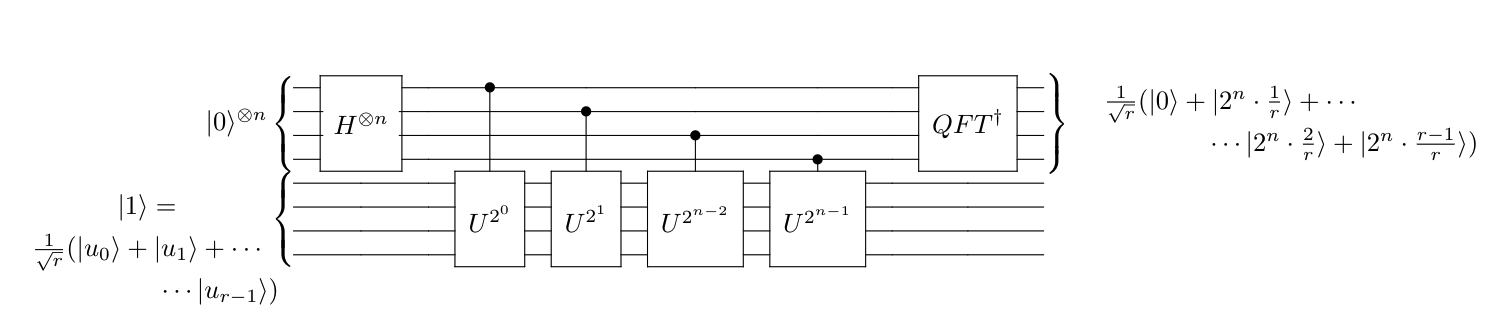
\includegraphics[scale=0.3]{../Graphics/shor_circuit.png}
    \caption{Algoritmo de Shor para la factorización de un número visto desde la estructura que propone Qiskit.}
    \label{fig:shorcircuit}
\end{figure}